\documentclass{cosas/tfg_domingo}
% \documentclass[numeros]{tfg_domingo}

\autor{Alejandro Martínez Floranes}
\titulo{Reescribir slatt en Python 3}
% Título corto para los encabezamientos de pagina:
\corto{} % En blanco si no es necesario recortarlo.
\ingles{Rewrite slatt in Python 3}
\fecha{julio de 2021}
% La normativa prescribe «cuatro o cinco palabras clave, en
% español y en inglés, para su indexación en el repositorio
% de TFG».
\palabras{reglas de asociación, hipergrafos, slatt, refactorizar}%
  {association rules, hypergraph, slatt, refactor}

\usepackage{lipsum} % Esto solo es relleno.
\usepackage{listings}
\usepackage{xcolor}
\usepackage{amssymb}

\definecolor{codegreen}{rgb}{0,0.6,0}
\definecolor{codegray}{rgb}{0.5,0.5,0.5}
\definecolor{codepurple}{rgb}{0.58,0,0.82}
\definecolor{backcolour}{rgb}{0.95,0.95,0.92}

\lstdefinestyle{mystyle}{
    %backgroundcolor=\color{backcolour},   
    commentstyle=\color{codegreen},
    keywordstyle=\color{magenta},
    numberstyle=\tiny\color{codegray},
    stringstyle=\color{codepurple},
    basicstyle=\ttfamily\footnotesize,
    breakatwhitespace=false,         
    breaklines=true,                 
    captionpos=b,                    
    keepspaces=true,                 
    numbers=left,                    
    numbersep=5pt,                  
    showspaces=false,                
    showstringspaces=false,
    showtabs=false,                  
    tabsize=2
}

\lstset{style=mystyle}

\begin{document}

% Si alguna palabra se divide entre dos líneas en un punto
% indebido, podemos indicar aquí los puntos de corte
% aceptables (si los hay), p. ej,
% \hyphenation{ba-rro-co, frío, cria-do, su-per-ra-tón}
\hyphenation{Dijkstra new-speak}

\portada
\frontmatter
% \sucinto{A Sofía}
\gracias{\input{cosas/agradecimientos.txt}}
\resumen{Las reglas de asociación son objetos matemáticos empleados de forma extensa en disciplinas como la minería de datos, aprendizaje automático y representación del conocimiento, entre otros campos.
Slatt es un proyecto de software libre desarrollado por José Luis Balcázar (Universidad Politécnica de Barcelona). Ofrece funcionalidades para el cálculo de reglas de asociación. Para ello, se apoya en implementaciones del algoritmo a priori para el cálculo de clausuras, el retículo de las clausuras y, entre otras
funcionalidades,devuelve las reglas representativas para cualquier elección de los parámetros de soporte y confianza.

En este proyecto, se ha mejorado este software utilizando como base las implementaciones disponibles en Slatt aplicadas a:

\begin{itemize}
    \item hipergrafos y algoritmos con aplicación a estos objetos;
    
    \item cálculo de clausuras y retículos (lattices);
\end{itemize}


Este trabajo ha requerido la búsqueda y análisis de algoritmos propuestos en la literatura científica sobre los puntos anteriores.
El lenguaje de desarrollo será Python3, encontrándose la implementación anterior en Python 2.7
%
% Conviene evitar aquí las llamadas a la bibliografía del
% trabajo, ya que el resumen tiene entidad independiente.
%

%% Aportamos nuestra perspectiva sobre la pertinencia de las
%% instrucciones {\tt goto}.


%%Pasar a tiempo presente
}{Association rules are mathematical objects used extensively in disciplines such as data mining, machine learning, and knowledge representation, among other fields.
Slatt is a free software project developed by José Luis Balcázar (Polytechnic University of Barcelona). It offers functionalities for the calculation of association rules. To do this, it relies on implementations of the a priori algorithm for the calculation of closures, the lattice of closures and, among others
functionalities, returns the representative rules for any choice of support and trust parameters.

In this project, this software has been improved using as a basis the implementations available in Slatt applied to:

\begin{itemize}
    \item hypergraphs and algorithms with application to these objects;
    
    \item calculation of closures and lattices (lattices);
\end{itemize}


This work has required the search and analysis of algorithms proposed in the scientific literature on the previous points.
The development language will be Python3, the previous implementation being in Python 2.7
}
\tableofcontents

\mainmatter
\chapter{\emph{Introducción}}

\section{Reglas de asociación}

Este proyecto se basa principalmente en reescribir \textbf{slatt} en Python 3 e incluir diferentes mejoras en el código para mejorar tanto su eficiencia en cuanto a rendimiento, como en reducción de lineas de código, y realizar una mejora en la legibilidad del propio código.

Slatt es un proyecto de software libre que ofrece funcionalidades para el cálculo de reglas de asociación. 

Las reglas de asociación son declaraciones 'if-then' que ayudan a mostrar la probabilidad de relaciones entre elementos de datos, dentro de grandes conjuntos de datos. Las medidas de evaluación  de las reglas de asociación son: \textit{el soporte, la confianza y el lift.} 

\begin{itemize}
    \item El \textbf{soporte} es la fracción de las transacciones que contiene tanto a X como a Y. 
    \item La \textbf{confianza} es la fracción de las transacciones en las que aparece X que también incluyen a Y; esto es, la confianza mide con que frecuencia aparece Y en las transacciones que incluyen X.
    \item El \textbf{lift} es la confianza de la reglas dividido por el cociente del consecuente.
\end{itemize}

\begin{figure}[ht!] % [h!] fuerza que el elemento se sitúe
                    % en la posición señalada, en vez de al
                    % comienzo de una página.
\begin{center}
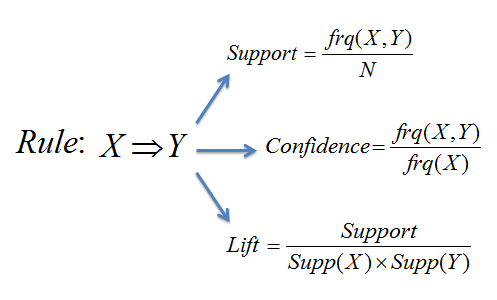
\includegraphics[width=.49\linewidth]{imagenes/AR_1.png}
\end{center}
\caption{Association Rules}
\label{fig_pro}
\end{figure}

A su vez, a la hora de plantear un problema utilizando reglas de asociación necesitamos disponer de diferentes elementos: 

\begin{enumerate}
    \item \textbf{Itemset.- }Conjunto de uno o más items (artículos).
    \item \textbf{K-itemset.- } Itemset con k elementos.
    \item \textbf{Soporte de un itemset.- } Fracción de las transacciones que contienen el itemset.
    \textbf{Itemset Frecuente} Itemset con soporte igual o superior a un umbral de soporte establecido por el usuario.
    \item \textbf{Umbral mínimo de confianza y de soporte.- } estos umbrales se utilizan para coger las reglas cuyo soporte o confianza sean mayores que las de umbral mínimo.
\end{enumerate}

Ejemplo sencillo de como utilizar las reglas de asociación para un problema general (problema de la lista de la compra). \citep{berzal2016reglas}

\begin{table}[h]
\centering
\begin{tabular}{|l|l|l|}
\hline
TID & Artículos                     \\ \hline
1         & Pan, leche, huevos            \\ \hline
2         & Pan, pañales, cerveza            \\ \hline
3         & Leche, pañales, cerveza            \\ \hline
4         & Pan, leche, pañales, cerveza         \\ \hline
5         & Pan, leche, huevos, cerveza         \\ \hline
\end{tabular}
\caption{Problema reglas de asociación}
\label{tab:my-table}
\end{table}

\begin{itemize}
    \item El \textbf{soporte} de la cerveza, supp(cerveza) = 4/5 = 0.8
    
    \item El \textbf{soporte} de los pañales, supp(pañales) = 3/5 = 0.6
    
    \item El \textbf{soporte} de la cerveza y los pañales, supp(cerveza,pañales) = 3/5 = 0.6
    
    \item La \textbf{confianza} entre la cerveza y los pañales seria, supp(cerveza,pañales) / supp(cerveza) 
   
    = 0.6 / 0.8 = 0.75
\end{itemize}

Para implementar este tipo de operaciones en código python, Slatt se basa principalmente en el algoritmo \textit{Apriori}, el proceso de este algoritmo sigue dos pasos: \citep{morales2013reglas}

\begin{enumerate}
    \item Genera los itemsets.
    \begin{itemize}
        \item Genera todos los itemsets con un elemento.
        \item Usa estos para generar los de dos elementos, y así sucesivamente.
        \item Toma todos los que cumplen con el mínimo soporte (esto permite eliminar posibles combinaciones).
    \end{itemize}
    \item Genera las reglas revisando que cumplan con el criterio mínimo de confianza.
\end{enumerate}

\lstinputlisting[language=python,caption=\textbf{Apriori Algorithm pyhton version},frame=bottom]{codigo/apriori.py}




% Utilice «citet» para integrar el nombre del autor en el
% texto. Para referencias aisladas, «citep».

\newpage
\section{Metodología y Requisitos}

Para la realización del proyecto se ha utilizado una metodología incremental, debido a que dicho proyecto esta dividido en diferentes partes, las cuales unas no tienen relación directa con otras, es por esto, que he decidió usar este tipo de metodología.

\begin{figure}[ht!] % [h!] fuerza que el elemento se sitúe
                    % en la posición señalada, en vez de al
                    % comienzo de una página.
\begin{center}
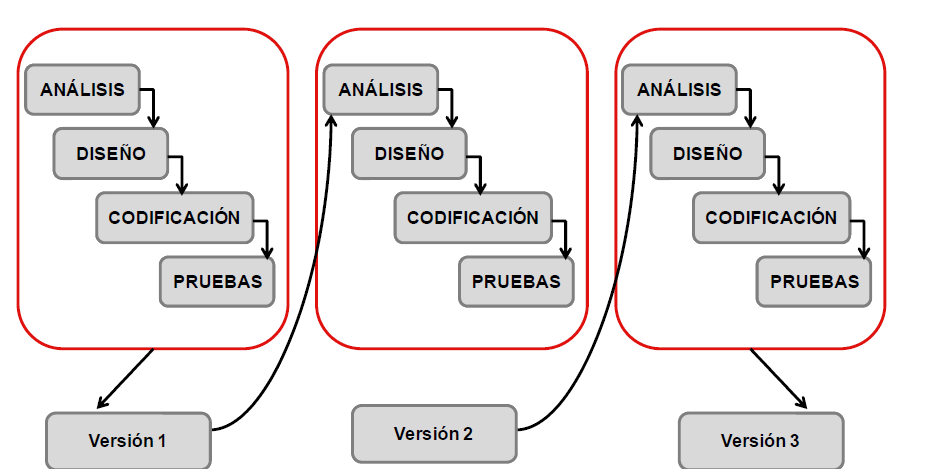
\includegraphics[width=.6\linewidth]{imagenes/Metodologia.png}
\end{center}
\caption{Metodología iterativa incremental}
\label{fig_pro}
\end{figure}

A continuación, defino los requisitos funcionales y no funcionales del proyecto software, al no ser una aplicación destinada hacia un usuario(cliente), los requisitos no funcionales, se basan en el correcto funcionamiento de la aplicación y los requisitos funcionales

\begin{table}[h]
\centering
\begin{tabular}{|l|l|}
\hline
Identificador & Descripción                     \\ \hline
RF01         & La aplicación deberá            \\ \hline
RF02         & La mejora en python3            \\ \hline
RF03         & La mejora en python3            \\ \hline
RF04         & La refactorización de l         \\ \hline
\end{tabular}
\caption{Requisitos funcionales del proyecto}
\label{tab:my-table}
\end{table}

\begin{table}[h]
\centering
\begin{tabular}{|l|l|}
\hline
Identificador & Descripción                              \\ \hline
RFN01         & La aplicación deberá tener la misma funcionalidad tanto en python2 como en python3                                          \\ \hline
RFN02          & La mejora en python3 deberá ser mas eficiente que la de su anterior versión                                                  \\ \hline
RFN03          & La mejora en python3 deberá tener menos lineas de código que su anterior versión                                         \\ \hline
RFN04          & La refactorización de los métodos no supondrá un cambio en los resultados                                               \\ \hline
\end{tabular}
\caption{Requisitos no funcionales del proyecto}
\label{tab:my-table}
\end{table}

\newpage

\chapter{\emph{Metaprogramación}}

\section{Conceptos básicos}
En este proyecto se van a utilizar diferentes herramientas relacionadas con la metaprogramación en el entorno de desarrollo.

La metaprogramación consiste en escribir programas que manipulan otros programas, es decir, cuando un programa es capaz de recibir una entrada, modificar el contenido de dicha entrada durante su ejecución y producir como salida otro programa, es un metaprograma.

La metaprogramación se base en estos conceptos principales:

\begin{itemize}
    \item \textbf{Reflexión.- } La capacidad de un programa para observar y modificar su estructura.
    
    Un ejemplo de reflexión seria cuando el código fuente de un programa se compila, se suele perder información sobre la estructura del programa, pero si un sistema permite reflexión, se mantiene dicha estructura como metadatos en el programa generado.
    
    La reflexión se puede descomponer en dos partes:
    
    \begin{enumerate}
        \item \textbf{Introspección.- } La capacidad de un lenguaje de obtener información sobre si mismo.
        
        Un ejemplo de introspección seria java, en java se puede saber hasta nivel del método cuantos atributos, que tipos utiliza, etc.
        \item \textbf{Intercesión.- } La capacidad de modificar el propio comportamiento/ significado de la estructura del programa.
    \end{enumerate}
    
    \item \textbf{Reificación.- } La capacidad de convertir algo abstracto en un dato explícito.
    Ejemplos de reificación serian:
    \begin{itemize}
        \item Crear un tipo de satos para acceder a una posición de memoria
        \item Crear estructuras de datos que representan tipos abstractos de datos
    \end{itemize}
\end{itemize}

En conclusión la metaprogramación es la programación que utiliza los programas como datos y permite modificar su propia estructura. \citep{silva2018metaprogramacion}

\section{Charla metaprogramación David Bleazley}

David Bleazley en esta charla explica uno de los grandes cambios que existen en Python3 respecto de Python2, la metaprogramación.\citep{David}

En concreto, explica como funcionan los decoradores, la clase \textit{decorators}, los descriptores y las metaclases, estos elementos son usados en este proyecto para mejorar el rendimiento de slatt y reducir a su vez lineas de código.

\subsection{Metaclases}
Una clase es un objeto que se utiliza para crear instancias de nuevos objetos.
Una metaclase está por encima de una clase. Agrupa un conjunto de clases, es decir, podemos tener metainformación sobre clases dentro de una metaclase. Es importante saber que en Python todo es un objeto, incluidas las clases, y cada una de las clases es creada por una metaclase.

\hfill

Por ejemplo:

\begin{verbatim}
def prueba_metaprogramacion():
class Prueba_met:
    pass
return Prueba_met

print(type(prueba_metaprogramacion))
print(type(prueba_metaprogramacion()))
\end{verbatim}

En el primer print la terminal no devuelve: \textit{<class 'function'>}, debido a que $prueba\_metaprogramacion$ pertenece a la clase función. Mientras que en el segundo de los print la terminal devuelve: \textit{<class 'type'>}, debido a que el retorno de $prueba\_metaprogramacion()$ pertenece a la clase tipo.

La clase type es una metaclase. Esta clase se usa para crear otras clases en Python. El constructor de dicha clase se usa para crear clases que pueden crear instacias de dicha clase.

\begin{verbatim}
##El constructor de la clase type tiene esta estructura

type(cls, what, bases=None, dict=None)
El primer parametro es el nombre de la clase
El segundo parametro es una tuple de clases base
El tercer parametro es un diccionario de llaves y valores,
es decir, la implementación de la clase.
\end{verbatim}

Cuando creamos una metaclase que hereda la clase tipo, esta tiene accesso al nombre de la clase, sus padres y todos sus atributos.

\subsection{Clase Type}
$\_\_new\_\_()$ es otro ejemplo de metaprogramación. Crea nuevas instancias de clase y no está vinculado a una instancia de la clase. Este método se llama antes de llamar a $\_\_init\_\_()$. Podemos anular el $\_\_new\_\_()$ de la superclase.
El retorno del método $\_\_new\_\_()$ es la instancia de la clase. Esto es útil cuando queremos modificar la creación de tipos de datos inmutables como las tuplas.

En este proyecto utilizamos este tipo de funcionalidad en la clase decorator.py la cual tiene una clase llamada StructMeta la cual hereda de type e implementa el funcionamiento de el metodo $\_\_new\_\_()$.
\begin{verbatim}
class StructMeta(type):
def __new__(cls, name, bases, clsdict):
    clsobj = super().__new__(cls, name, bases, clsdict)
    sig = make_signature(clsobj._fields)
    setattr(clsobj, '__signature__', sig)
    return clsobj
\end{verbatim}

\subsection{Usos de la Metaprogramación}

\begin{enumerate}
    \item Si queremos comprobar si una clase esta definida correctamente, podemos usar metaclases.
    \item Podemos usar metaclases para generar errores durante la importación de los módulos de la clase.
    \item Podemos usar la metaprogramación si queremos que nuestras clases tengan una convención especifica de métodos y atributos.
    \item Las metaclases se pueden utilizar para modificar el atributo de clase.
    \citep{Farhad}
\end{enumerate}


\chapter{\emph{Hipergrafo y problemas relacionados}}

\section{Conceptos básicos}
En dicho proyecto también se van a tratar elementos como los hipergrafos
y algoritmos con aplicación a estos.

Un hipergrafo H es una familia de subconjuntos (aristas) de un conjunto finito de vértices. Un hipergrafo es simple si ninguno de sus bordes está contenido en ningún otro de sus bordes. Decimos que un hipergrafo está saturado si cada subconjunto del conjunto de vértices está contenido en un borde o contiene un borde de el hipergrafo. \citep{Thomas}

Se toma como algoritmo principal \textit{The algorithm of Berge}, al cual se le añadirán diferentes mejoras analizadas y comprobadas en el paper desarrollado por \citep{JGAA-107} el cual implementa un algoritmo eficiente para la generación transversal de hipergrafos.


% Añadiendo la opción «commandchars=\\\{\}», los caracteres
% \, { y } del archivo fuente se interpretan como código
% LaTeX y puede darse formato al código (manualmente). Hay
% que tener esto en cuenta cuando estos caracteres formen
% parte del código en sí.
%
% Sin esa opción, el fichero de reproduce tal cual.

\begin{center}
% Puede pasar parámetros al comando «VerbatimInput» del
% paquete «fancyvrb». Por ejemplo:


\lstinputlisting[language=python,caption=\textbf{Original Berge Algorithm},frame=bottom]{codigo/berge.py}

\lstinputlisting[language=python,caption=\textbf{Efficient Berge Algorithm},frame=bottom]{codigo/bergeMod.py}


%\codigo[numbers=none,frame=single]{codigo/berge.c}{Original}{11.5cm}

\end{center}

\section{Transversales mínimas de un Hipergrafo}

\newpage
\section{Problemas relacionados con SIMPLE-H-SAT en la teoria de bases de datos}

Siguiendo la lectura del paper \citep{Thomas} en el apartado séptimo habla sobre los diferentes problemas relacionados con el SIMPLE-H-SAT en la teoría de bases de datos.

Inicialmente, habla sobre las bases de datos relaciones y hace una explicación sobre como esta formada una relación, básicamente una
Una relación es una tabla de tuplas distintas de pares de componente que son valores de los dominios de los atributos. Por ejemplo, $U = \{A_0,A_1,...,A_n\}$ es un conjunto de atributos, cada uno de los cuales está asociado a un dominio D. Entonces $D(A_i)$ es el dominio de un atributo $A_i$. 
Entonces una relación sobre U es un subconjunto de $\prod_{i=1}^{n}D(A_i)$, y el los elementos de una relación se denominan tuplas.

El paper también habla sobre las relaciones funcionales, es decir, esas reglas de asociación que nos dan una información de unas variables frente a otras, y lo explica de la siguiente manera:

"Dados los conjuntos $ X, Y $ de atributos, la dependencia funcional (FD) $ X \rightarrow Y $ se mantiene en la relación R si en cada tupla los valores de los atributos en Y están determinados únicamente por los valores de los atributos en X, para tuplas $ t_1 , t_2 \in R \;; t_1 [X] = t_2 [X] $ implica que $ t_1 [Y] = t_2 [Y]: $ Dado que posiblemente todas las tuplas de una relación tienen los mismos valores para algún atributo, el lado izquierdo X de un FD $ X \rightarrow Y $ puede estar vacío. Si $Y \subseteq X$, entonces se llama dependencia funcional trivial."

Y en general, explica como conseguir relaciones funcionales válidas, para ello se tienen que definir diferentes términos.

\begin{itemize}
    \item \textbf{Conjuntos cerrados.-} Son los que no puedes ampliar sin perder soporte. Formalmente hablando, un conjunto $X \subseteq I$ es cerrado si $X=X$, donde $X$ es la clausura de $X$ y se calcula con la $formula :X=\{a \in I |s( X \cup\{a\}) = s(X)\}$
    
    \item \textbf{conjuntos frecuentes.-} $F_\tau=\{X \subseteq I \;|\; s(X) \geq \tau\}$
    \item \textbf{conjuntos frecuentes cerrados.-} $FC_\tau=\{X \in F_\tau \;|\; \forall Z \supset X,s(Z)<s(X)\}$
    \item \textbf{generadores minimales frecuentes.-} $\{X \in F_\tau \;|\; \forall Y \subset X,s(Y)>s(X)\}$
    
\end{itemize}

Con estos elementos definimos si una regla es redundante, sirve para no llenar la base de datos de una misma regla de asociación que se repite durante el tiempo, ocupa espacio innecesario y no ofrece ningún tipo de información valiosa.

Después de la definición de los anteriores conceptos, podemos decir  que una regla de asociación es:

$AR_\tau,_\gamma=\{X\rightarrow Y \;|\; s(X \rightarrow Y)\geq \tau,c(X \rightarrow Y) \geq \gamma\}$, siendo $\tau$ y $\gamma$ umbrales de soporte y confianza respectivamente.

También podemos definir la reglas representativas como:

$RR_\tau,_\gamma=\{r \in AR_\tau,_\gamma \;|\; \nexists \; r′ \in AR_\tau, \;|\; \gamma\{r\}$ tal que $r \in C(r′)\}$ \citep{UC}

Con esta definición de regla representativa no redundante podemos conseguir una cantidad de reglas de asociación menor con un mismo valor de contenido, es decir, nos ahorraríamos mucho espacio en una base de datos gracias a esta definición de regla representativa.








\chapter{\emph{KD Trees}}

\section{Conceptos básicos}

Un KD Tree (también conocido como K-Dimensional Tree) es un árbol de búsqueda binario donde los datos en cada nodo son un punto k-dimensional en el espacio. Básicamente, es una estructura de datos que utiliza una partición en el espacio para organizar puntos en un espacio K-Dimensional.

\begin{enumerate}
    \item Cada nodo tiene como clave multidimensional un vector de tamaño k
que contiene los valores de las k claves unidimensionales y tiene asociado un discriminante con valor entero entre 1 y k.
    \item Para cada nodo con clave multidimensional x y discriminante j se
cumple que cualquier nodo del subárbol izquierdo con clave multidimensional y cumple que su n-ésima componente es menor que la n-ésima componente de x, es decir (yn < xn ). Para el subárbol derecho se cumple que la n-ésima componente de la clave multidimensional z de cualquier nodo de este subárbol es mayor que la n-ésima componente de la clave x, es decir (zn > xn ).
    \item La raíz del kd-tree tiene profundidad 0 y discriminante 1. Cualquier
nodo a una profundidad p tiene discriminante de valor: (p mod k) + 1.
\citep{marti2010copy}
\end{enumerate}

Otra de las aplicaciones es la de representar un conjunto de puntos y la consulta más frecuente sobre este conjunto es la de localizar el punto o puntos más cercanos a uno dado. Esta consulta se conoce con el nombre de búsqueda del vecino más cercano.

\section{Implementación en Reglas de Asociación}

Los kd-trees son frecuentemente utilizados en bases de datos para satisfacer consultas que incluyan valores de varios campos. Esto se puede extrapolar a las reglas de asociación, ya que se podrían realizar consultas como se ha explicado en el ejemplo introductorio de reglas de asociación.

\hspace{0.5mm}

Una consulta podría ser por ejemplo, saber todos los registros de personas que compren pan, leche y huevos, y además tengan entre 25 y 45 años, y que vivan en España, todo esto se podría realizar en una única consulta utilizando los \textit{KD trees} como algoritmo de búsqueda ya que permite realizar diferentes consultas simultaneas, en lugar del algoritmo \textit{apriori} actualmente utilizado, en el que al añadir múltiples consultas, su coste computacional hace que no tenga sentido dicho calculo, debido a su lento proceso.

\newpage
\section{Ejemplo gráfico KD Tree}

\hfill

Ejemplo gráfico de un KD-tree para el siguiente ItemSet:

\textbf{{(3,6),(17,15),(13,15),(6,12),(9,1),(2,7),(10,19)}}

\hfill

\begin{figure}[h]
\begin{center}
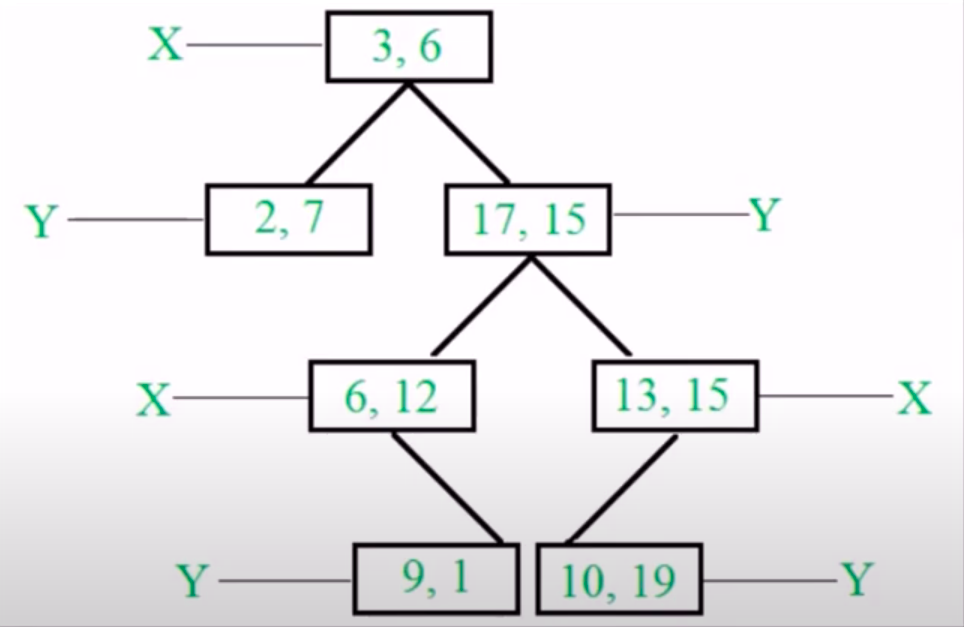
\includegraphics[width=.4\linewidth]{imagenes/kdtree1.png}
\end{center}
\caption{Árbol del ItemSet}
\label{arbol_kd}
\end{figure}

\begin{figure}[h]
\begin{center}
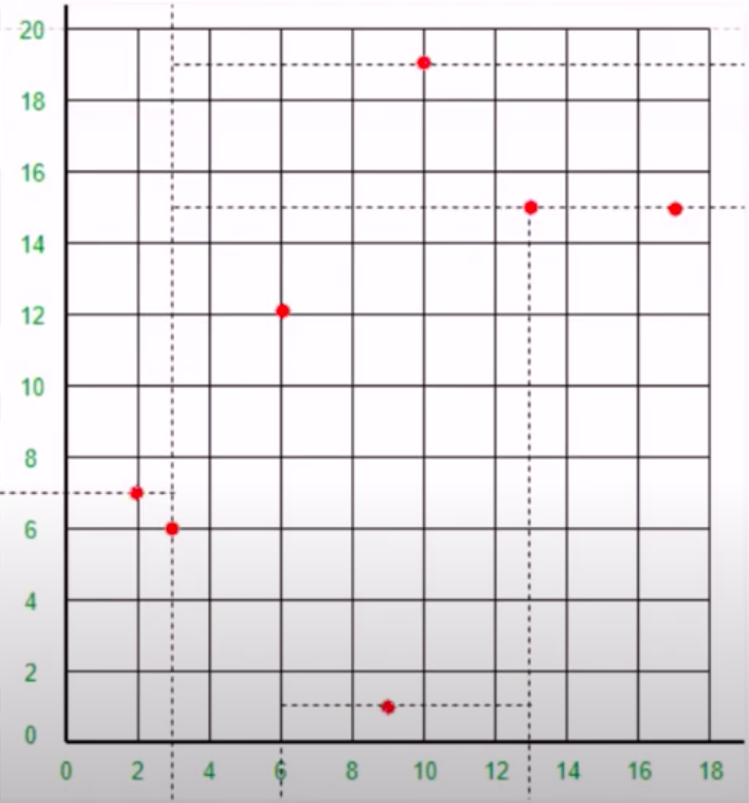
\includegraphics[width=.4\linewidth]{imagenes/kdtree2.png}
\end{center}
\caption{Gráfica del ItemSet}
\label{grafica_kd}
\end{figure}

Desde un punto de vista geométrico como se ve en la Ilustración \ref{arbol_kd}, cada nodo del kd tree hace una partición del plano en dos “subplanos”. En la Ilustración \ref{grafica_kd} todos los puntos en el “subplano” de la izquierda corresponden al subárbol izquierdo del nodo raíz, y los que quedan a la derecha son los puntos del subárbol derecho.


\chapter{\emph{Metodología test unitarios}}

En esta sección se especifica como se realizan los test unitarios, para comprobar si las dos versiones del código mantienen la misma funcionalidad basándose en la salida de estos test.

\hfill

\lstinputlisting[language=bash,caption=\textbf{Makefile},frame=bottom]{codigo/makefile}

Utilizando este \textbf{makefile} se realiza una ejecución simultanea de ambas versiones, guardando dicha salida en un fichero.txt y a continuación, se hace un \textbf{diff} entre los dos archivos, en el caso en el que el \textbf{diff} devuelva un archivo vacío, sabremos que las dos versiones tienen la misma funcionalidad.

% Indique aquí el fichero .bib que contenga su bibliografía.
\bibliography{refs}

\end{document}
